\chapter{The Lattice Boltzmann Algorithm}
As previously asserted, the heart of the Lattice-Boltzmann Algorithm lies on its discretization of the phase space\cite{franco} \cite{integerLatticeDynamics}. To discretize the phase space, one must first choose the region to simulate. In this work, we name the extremal values in the $k$ axis of the phase space $K_{min}$ and $K_{max}$. Then, one has to fix either the size of the grid or the size of the lattice. We named the size of the grid in the $k$ axis $N_k$ (i.e. $N_x$ or $N_{vz}$). The size of the lattice in the $k$ axis ($dk$) and the extremal values are related by: $$ dk = \frac{K_{max}-K_{min} }{N_k}  $$

In this work we are going to consider the canonical density-velocity phase space. Now that we have properly defined the phase space grid, we can proceed to the initialization. For simplicity, we choose gaussian initial conditions given by:
\begin{equation}
f(\vb{r},\vb{v})= A \exp{-\frac{\vb{r}^2}{\sigma_r^2} - \frac{\vb{v}^2}{\sigma_v^2}}
\end{equation}
Where $f(\vb{r},\vb{v})$ is the phase space, $A$ is an indirect measure of the total mass in the system, $\vb{r}$ is the vector = $(x,y,z)$, $\vb{v}$ is the vector = $(vx,vy,vz)$, and $\sigma_r$ and $\sigma_v$ are a measure of the width of the gaussian profile in the given axis. After initialization, the system evolves by classical mechanics and the modelling of the collisional step, which can be seen more easily in figure  \ref{flowchart}

\begin{figure}[H]
    \centering
    %\includegraphics[width=10cm,height =7cm]{Diapositiva1.jpg}
    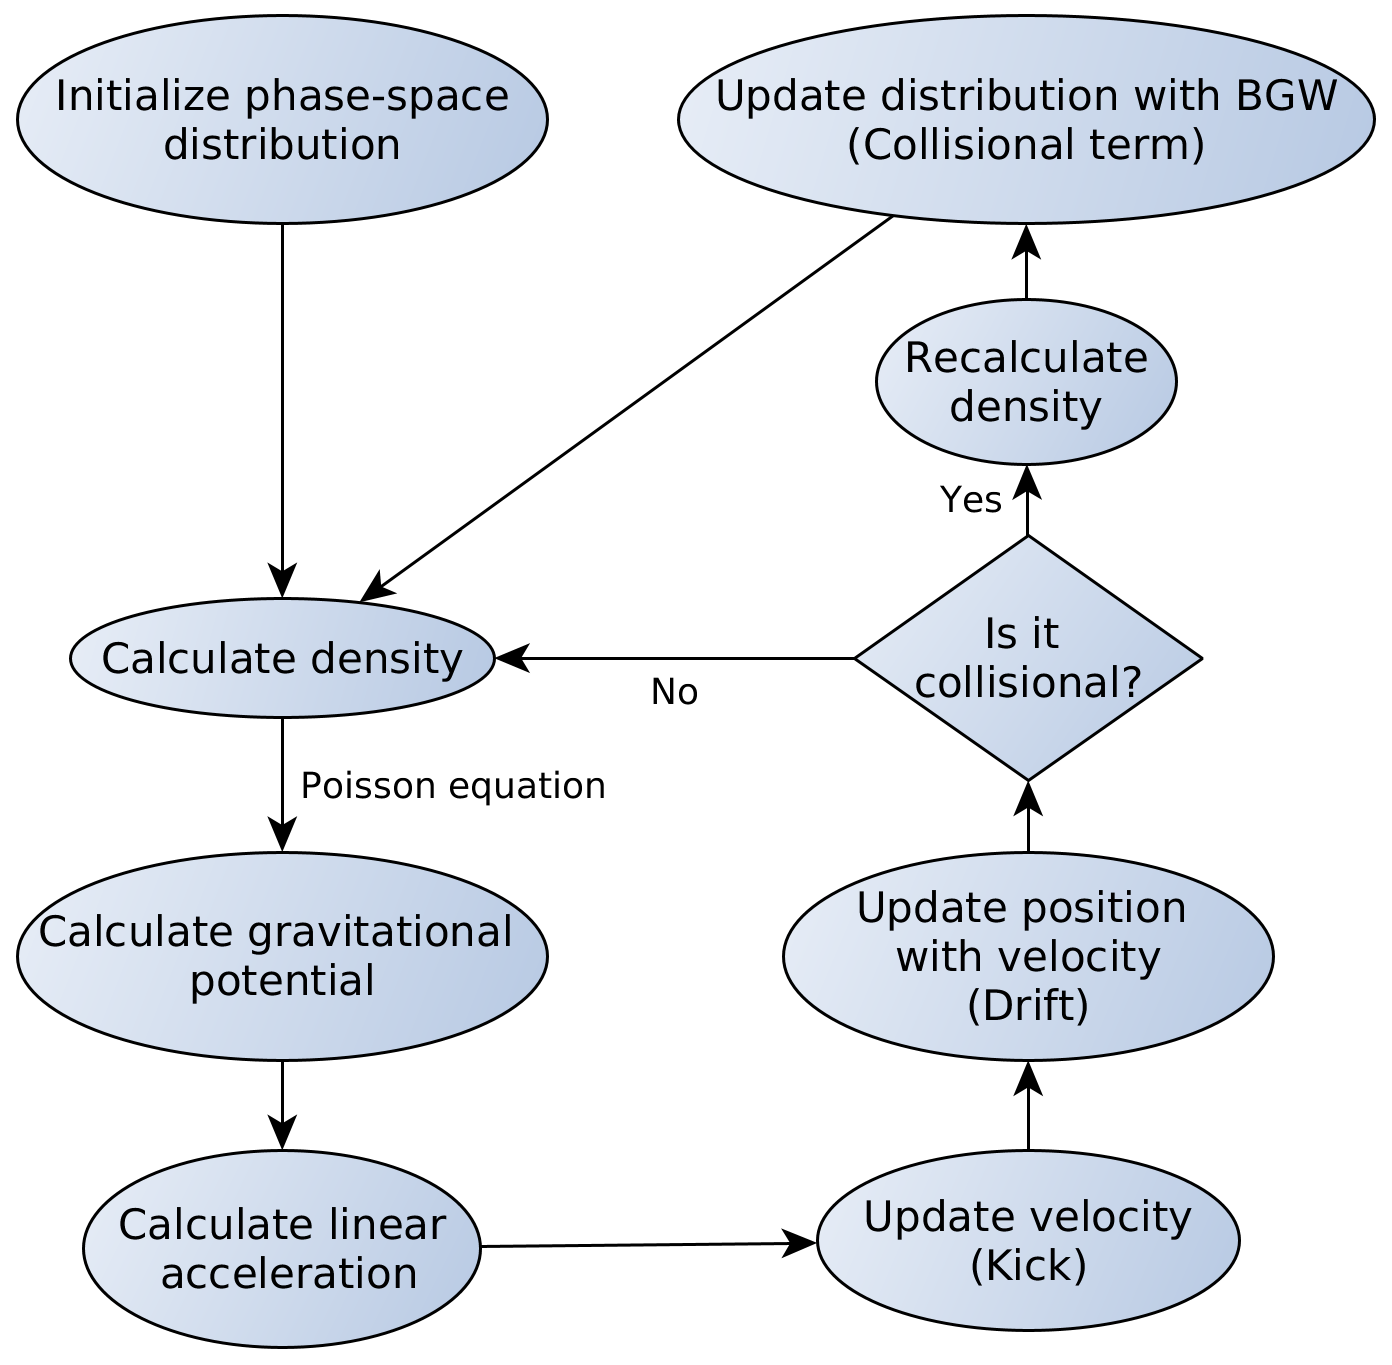
\includegraphics[scale=0.2]{imag/flowchart.png}
    \caption{Flowchat of the algorithm.}
    \label{flowchart}
\end{figure}

\section{The Mass Integral and the Poisson Equation}
asdfasdf
\section{Kick and Drift}
asd
\section{The Collisional Step}
asd
\section{Units and Initial Conditions}




















\chapter{Results}
\section{No Collisional}
\section{$\tau$ = 10}
\section{$\tau$ = 100}
\section{$\tau$ = 250}
\section{$\tau$ = 500}
\section{$\tau$ = 1000}
\section{Different Equlibrium Distributions}